\chapter*{Capitolo 2}
\addcontentsline{toc}{chapter}{Capitolo 2}

\section*{Tecnologie Utilizzate}
\addcontentsline{toc}{section}{Tecnologie Utilizzate}
In questa sezione si discuteranno le tecnologie utilizzate durante il progetto sia dal punto di vista software che hardware per entrambe le architetture RISC-V e x86\_64.

\section*{GCC}
\addcontentsline{toc}{section}{GCC}
Gnu C Compiler (GCC) \cite{GCC} è un compilatore per vari linguaggi di programmazione inizialmente rilasciato per fornire supporto di compilazione ai sistemi il sistema operativo GNU.\\
Dopo la compilazione del programma C viene prodotto un file output con le istruzioni assembly. Due compilati di due architetture diverse avranno peso, complessità e struttura diversi.\\
\newline
È inoltre possibile compilare degli eseguibili con GCC con delle specifiche flag per attivare / disattivare delle funzionalità specifiche del compilatore. Durante l'attività di tesi è stato utilizzato al fine di produrre e comparare eseguibili per i due tipi di architettura al fine di paragonarne il codice assembly.\\
Un esempio di compilazione con tutte le flag di sicurezza disabilitate al fine di eseguire un attacco buffer overflow è il seguente
\begin{minted}{c}
gcc vuln.c -fno-stack-protector -z execstack -no-pie -Wl, norelro -o riscv_bof.out
\end{minted}
In questo caso viene disabilitato lo stack protector, il bit NX, la randomizzazione degli indirizzi e la Global Offset Table (GOT) \cite{CTF101got} viene impostata come ``read only".
\section*{GDB}
\addcontentsline{toc}{section}{GDB}
GNU Debugger (GDB) \cite{GDB} è un debugger originario del sistema operativo GNU, sviluppato da Richard Stallman e utile a eseguire debugging su codice compilato. Grazie a GDB è possibile eseguire step by step le istruzioni macchina che vengono eseguite dal calcolatore, inserire breakpoint, disassemblare funzioni e vedere lo status dei registri ad un determinato istante di esecuzione. Durante l'attività di tesi è stato utilizzato un flavour di GDB conosciuto con il nome di GEF \cite{GEF}.
\vspace{1cm}
\FloatBarrier
\begin{figure}[!htbp]
    \centering
    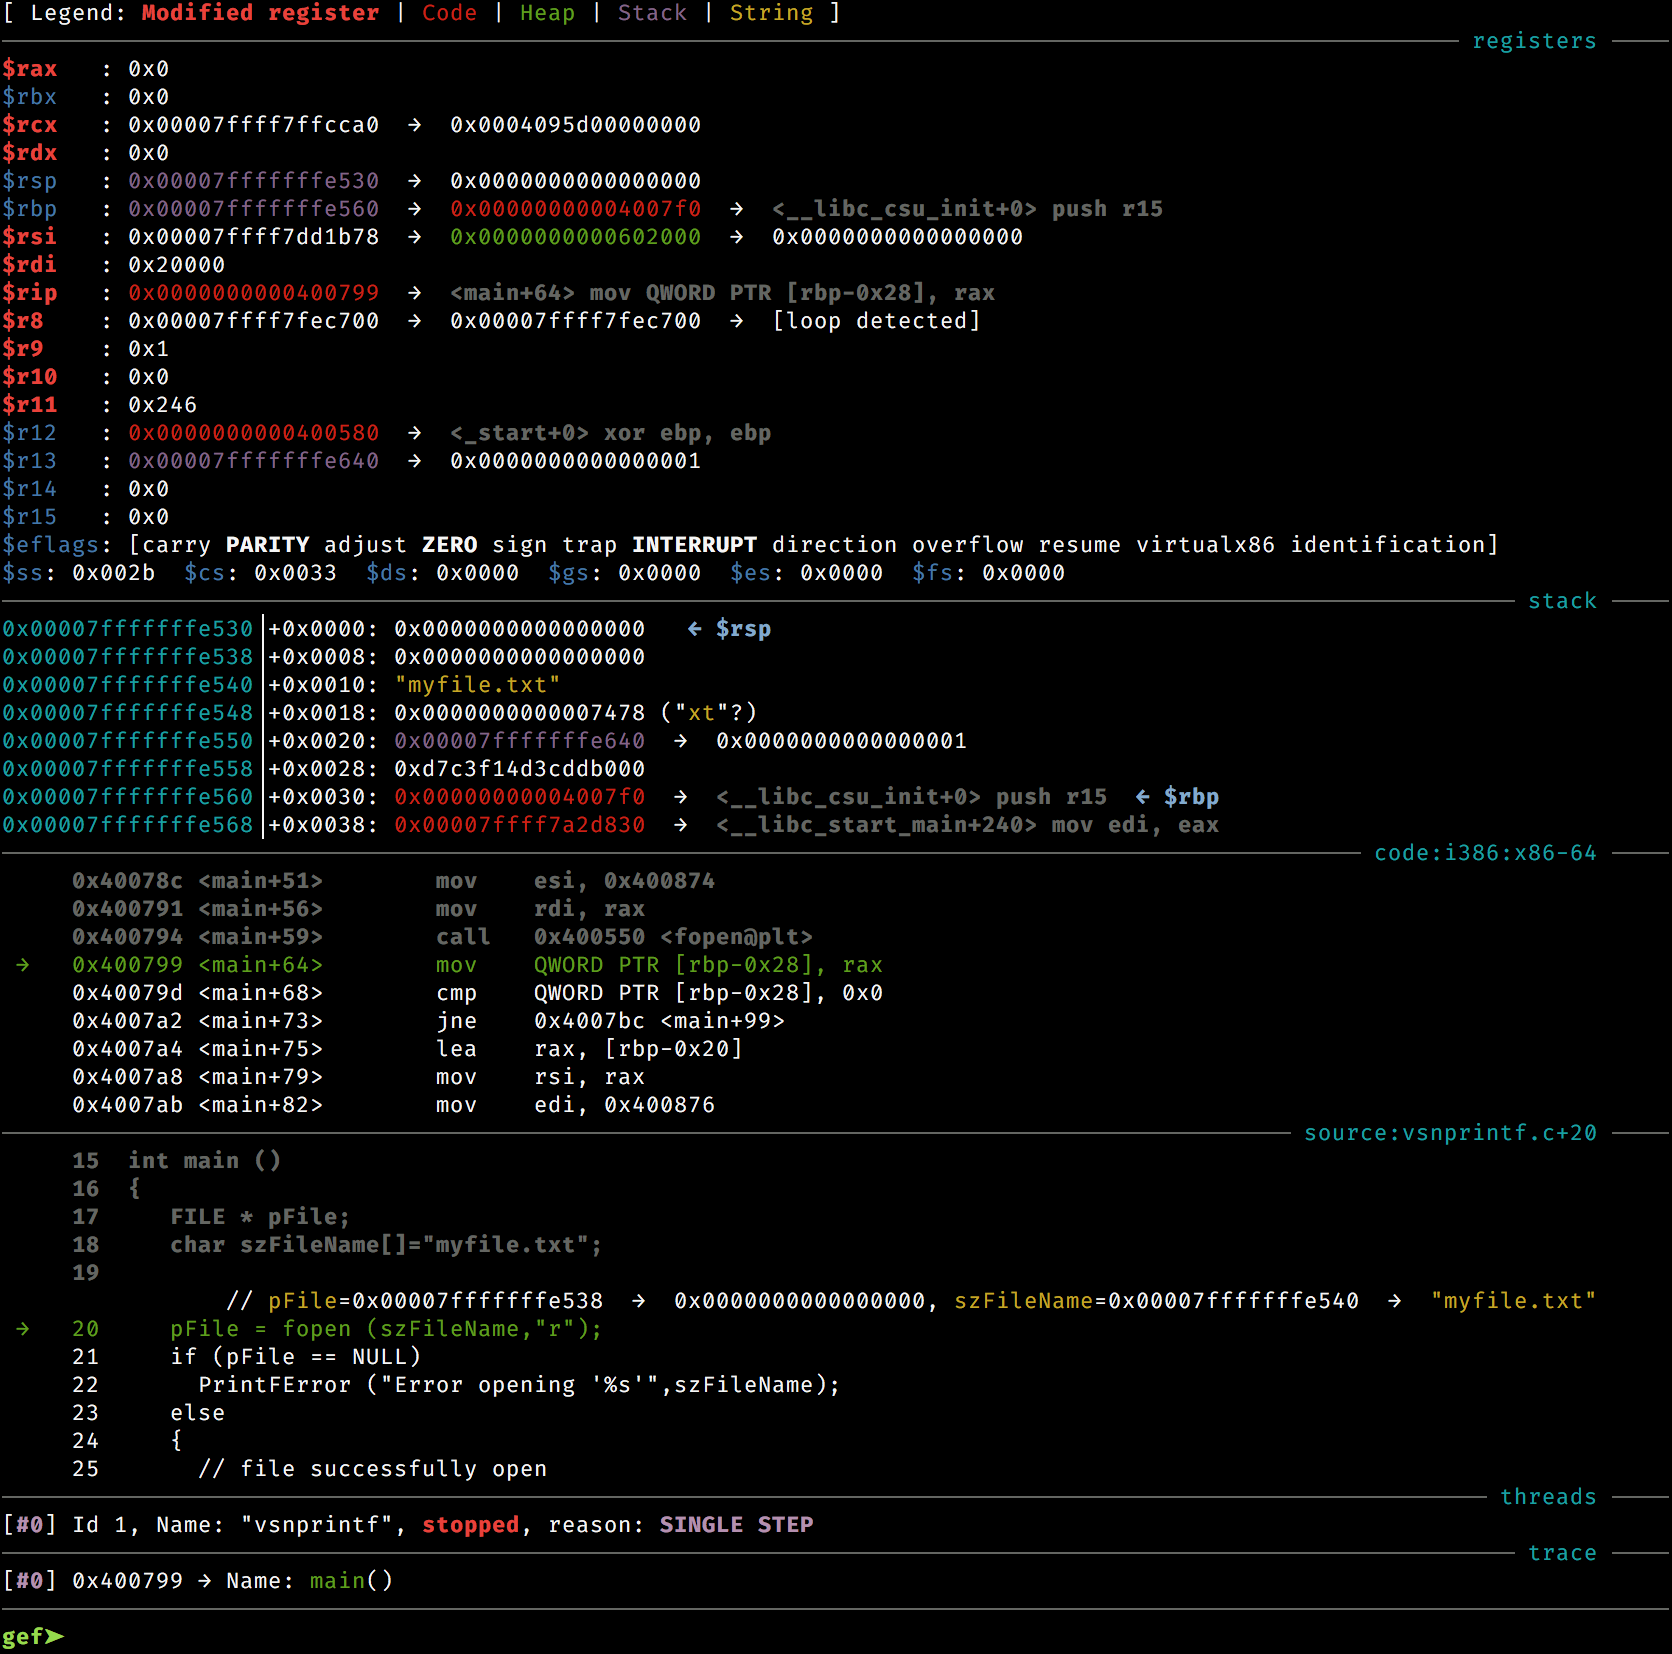
\includegraphics[width=0.57\linewidth]{images/gef.png}
    \caption{GEF in esecuzione} 
\end{figure}
\FloatBarrier
\vspace{1cm}
\section*{Differenza di compilati}
\addcontentsline{toc}{section}{Differenza di compilati}
Compilando con GCC un semplice ``hello world" notiamo già da subito una differenza sostanziale: il peso in byte del programma compilato è quasi la metà in architettura RISC-V.\\
Su x86\_64 abbiamo infatti un peso complessivo del programma di 15952 byte, contro un totale di 8472 byte per il programma compilato per RISC-V.\\
Questo a prima vista può sembrare inutile al fine dell'attacco, bisogna però pensare alla quantità di istruzioni utili e path di attacco che il binario può offrirci. Avendo meno byte e quindi meno istruzioni in primo luogo è più difficile poter eseguire un attacco dato che il programma offrirà meno vettori di attacco e, in caso di return oriented programming, meno gadget. 
\begin{center}
\begin{tabular}{| c | c c c|} 
 \hline
 \textbf{Arch} & \textbf{GCC Version} & \textbf{OS} & \textbf{Size in B} \\ [0.5ex] 
 \hline\hline
 X86\_64 & 13.2.0 & 24.04 LTS LTS & 15952 \\ 
 \hline
 RISC-V & 11.4.0 & Ubuntu 22.04.4 LTS & 8472 \\
 \hline
\end{tabular} 
\end{center}
Il risultato del compilato è il seguente, per entrambe le architetture\\
\newline
\textbf{x86\_64}
\begin{minted}{c}
ELF 64-bit LSB pie executable, x86-64, version 1 (SYSV), dynamically linked, interpreter
/lib64/ld-linux-x86-64.so.2, BuildID[sha1]=2c0422d81d038623388b83cac19defb8954052ad,
for GNU/Linux 3.2.0, not stripped
\end{minted}
\textbf{RISC-V}
\begin{minted}{c}
ELF 64-bit LSB pie executable, UCB RISC-V, RVC, double-float ABI, version 1 (SYSV),
dynamically linked, interpreter /lib/ld-linux-riscv64-lp64d.so.1, 
BuildID[sha1]=fa13aed56cf533eead5c256e3d79da49c0637a1f, for GNU/Linux 4.15.0, not stripped
\end{minted}
\section*{SiFive Cluster}
\addcontentsline{toc}{section}{SiFive}
Per svolgere i test, si sono utilizzati più tipi di processori basati su architettura RISC-V. Il primo tra questi è il cluster del Monte Cimone \cite{mcimone} il quale è un HPC che monta un SoC \textit{SIFIVE FREEDOM U740} e 16 GB di memoria.
\vspace{1cm}
\FloatBarrier
\begin{figure}[!htbp]
    \centering
    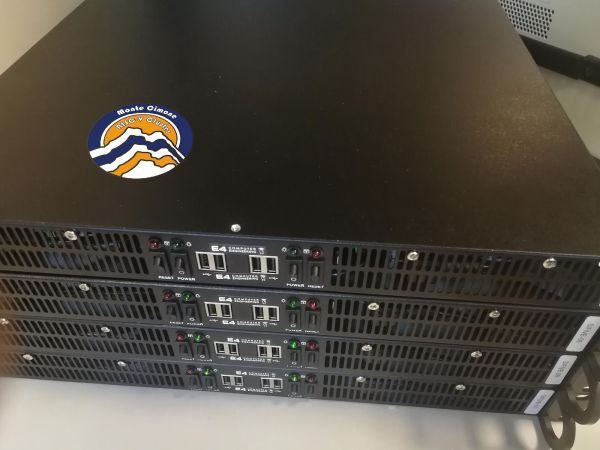
\includegraphics[width=1\linewidth]{images/cluster-monte-cimone-risc-v.jpg}
    \caption{Cluster RISC-V del Monte Cimone} 
\end{figure}
\FloatBarrier
\vspace{1cm}
Questo SoC ha alcune feature di sicurezza che sono state testate durante il progetto, come ad esempio la mancanza di speculative execution \cite{Techtarget} che rende il processore non vulnerabile a determinati tipi di attacchi che verranno descritti in seguito.\\
\newline
Nonostante per alcuni tipi di attacco sia cruciale il tipo di SoC montato, per gli attacchi come buffer overflow e return oriented programming è necessario solo avere l'ISA di base con le istruzioni principali. Ogni altra implementazione microarchitetturale non può arginare facilmente questa tipologia di attacchi alla memoria, a meno che non si implementi qualcosa di più sofisticato come l'utilizzo che viene fatto da Apple di puntatori cifrati \cite{AppleSec}, che però necessitano di modifiche lato hardware da implementare nel chip. 
\section*{MILK-V Board}
\addcontentsline{toc}{section}{MILK-V}
Una soluzione più economica ad un cluster HPC basato su RISC-V sono dei SoC basati su chip RISC-V a basso costo montati su dei Single Board Computer (SBC).\\ 
Le due schede utilizzate sono state Milk-V Duo S dotato di un SoC SG2000 con un processore RISC-V C906, 512MB di memoria e un MILK-V Duo 256M con SoC SG2002, processore C906 e 256MB di memoria.\\
Durante la fase di test si è potuto constatare che i test sulle due schede, basandosi allo stesso processore restituiscono risultati identici, quindi è stato scelto di proseguire sulla prima scheda perché più performante.
\newpage
\FloatBarrier
\begin{figure}%
    \centering
    \subfloat{{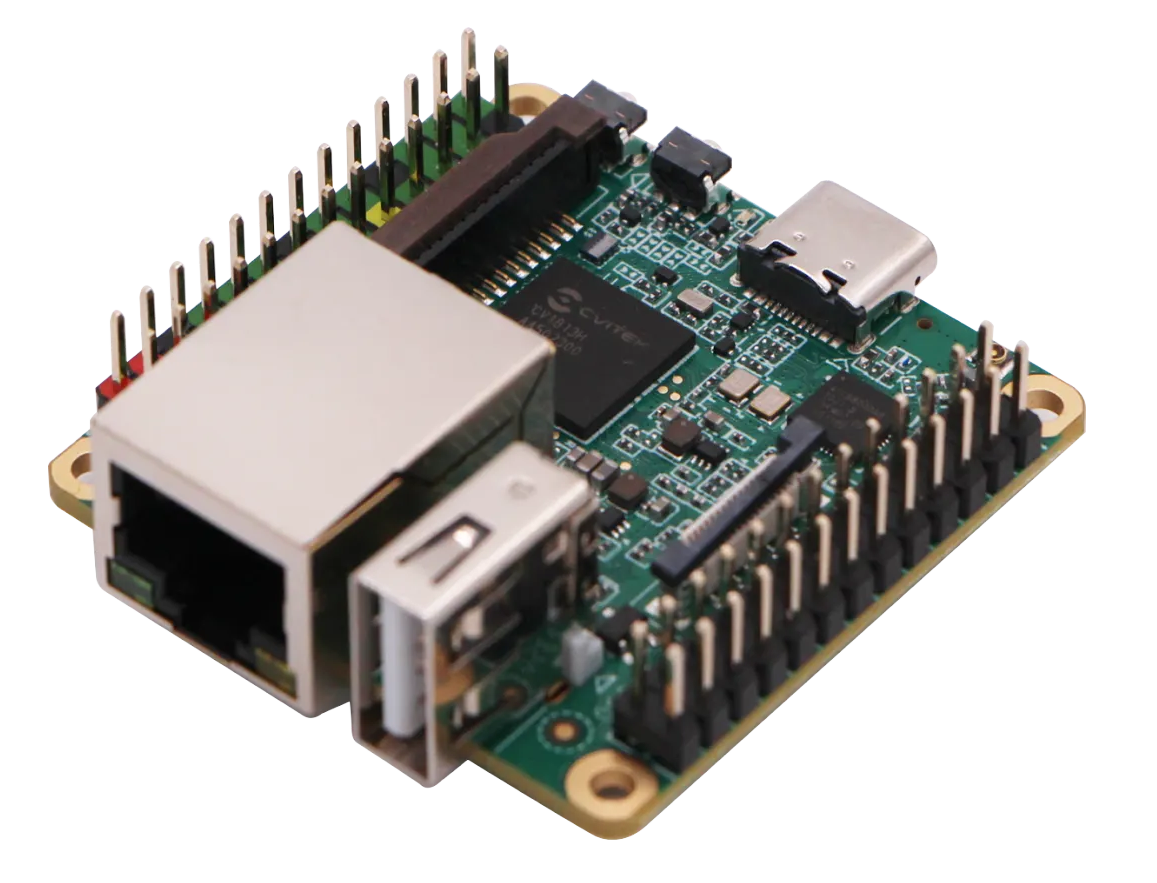
\includegraphics[width=6cm]{images/duos-side.png} }}%
    \qquad
    \subfloat{{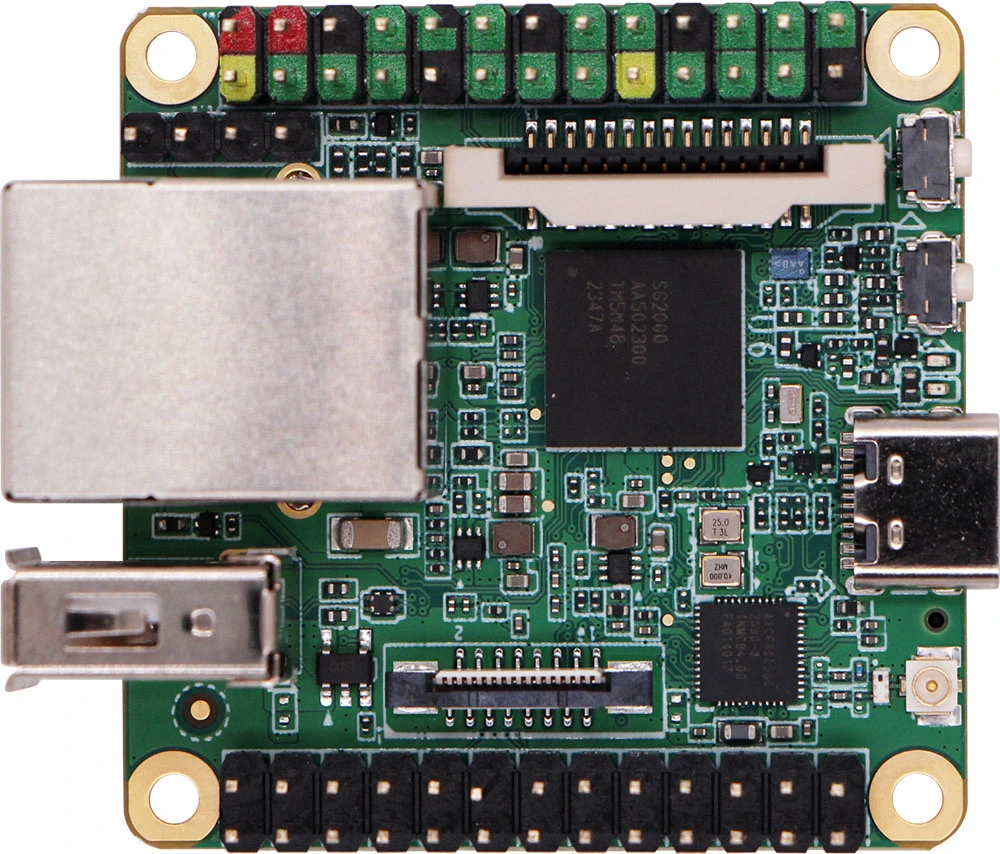
\includegraphics[width=5cm]{images/duos-top.png} }}%
    \caption{MILK-V Duo S}%
\end{figure}
\begin{figure}%
    \centering
    \subfloat{{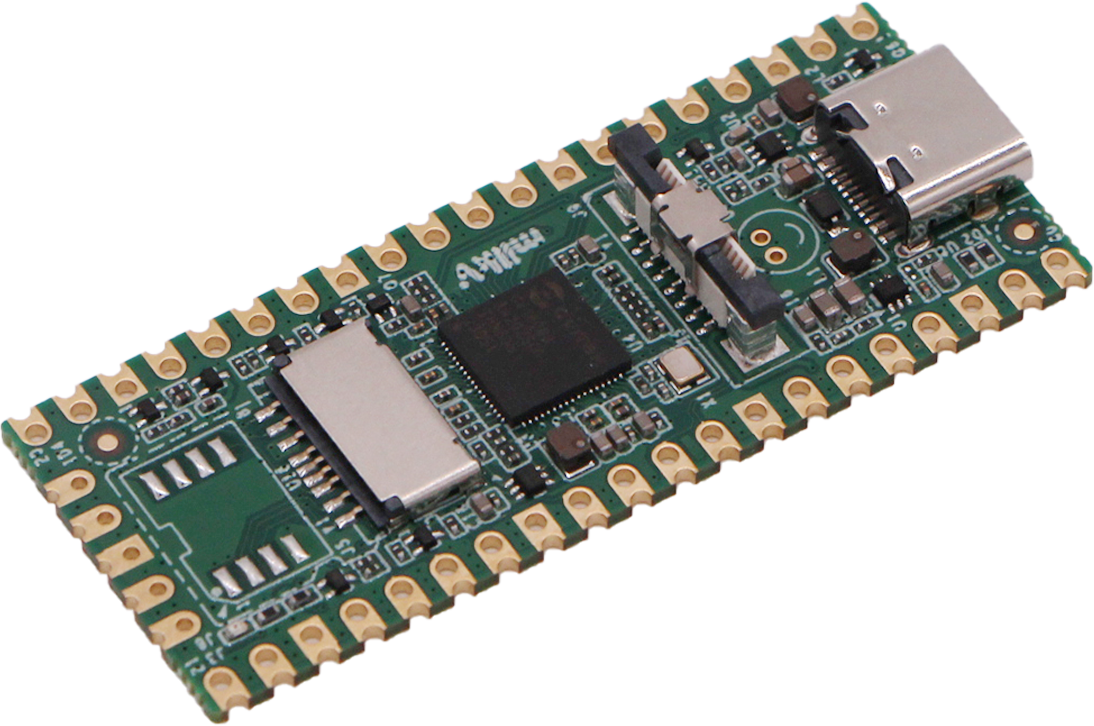
\includegraphics[width=7cm]{images/duo-side.png} }}%
    \qquad
    \subfloat{{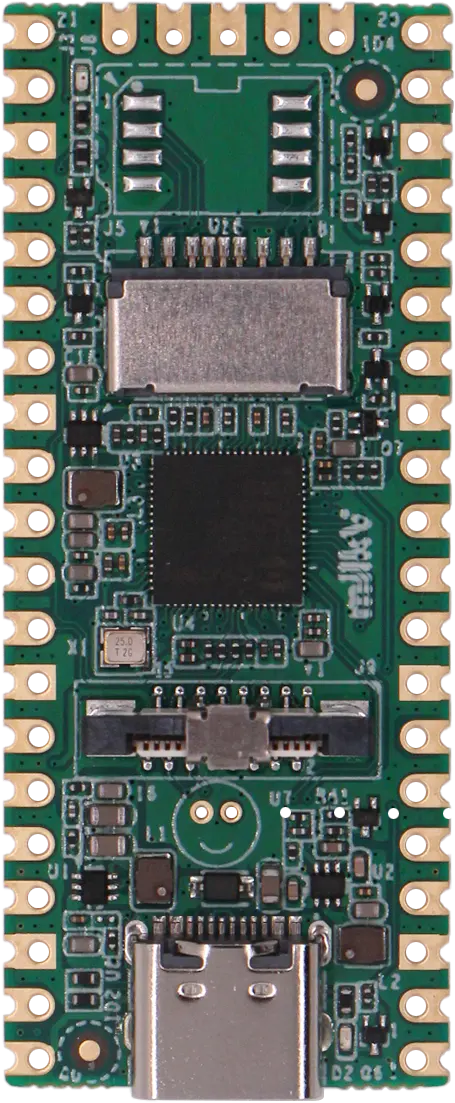
\includegraphics[width=2cm]{images/duo-top.png} }}%
    \caption{MILK-V Duo}%
\end{figure}
\FloatBarrier
\newpage
Nella figura \ref{ref:duo-pinout} è presentato il pinout della scheda Milk-V. Si sottolinea la presenza di pin GPIO, ovvero pin general purpose interfacciabili con un eventuale sistema Linux che si possono pilotare scrivendo su file. Più avanti si vedrà un attacco a questo tipo di pin usando un buffer overflow.
\vspace{1cm}
\FloatBarrier
\begin{figure}[!htbp]
    \centering
    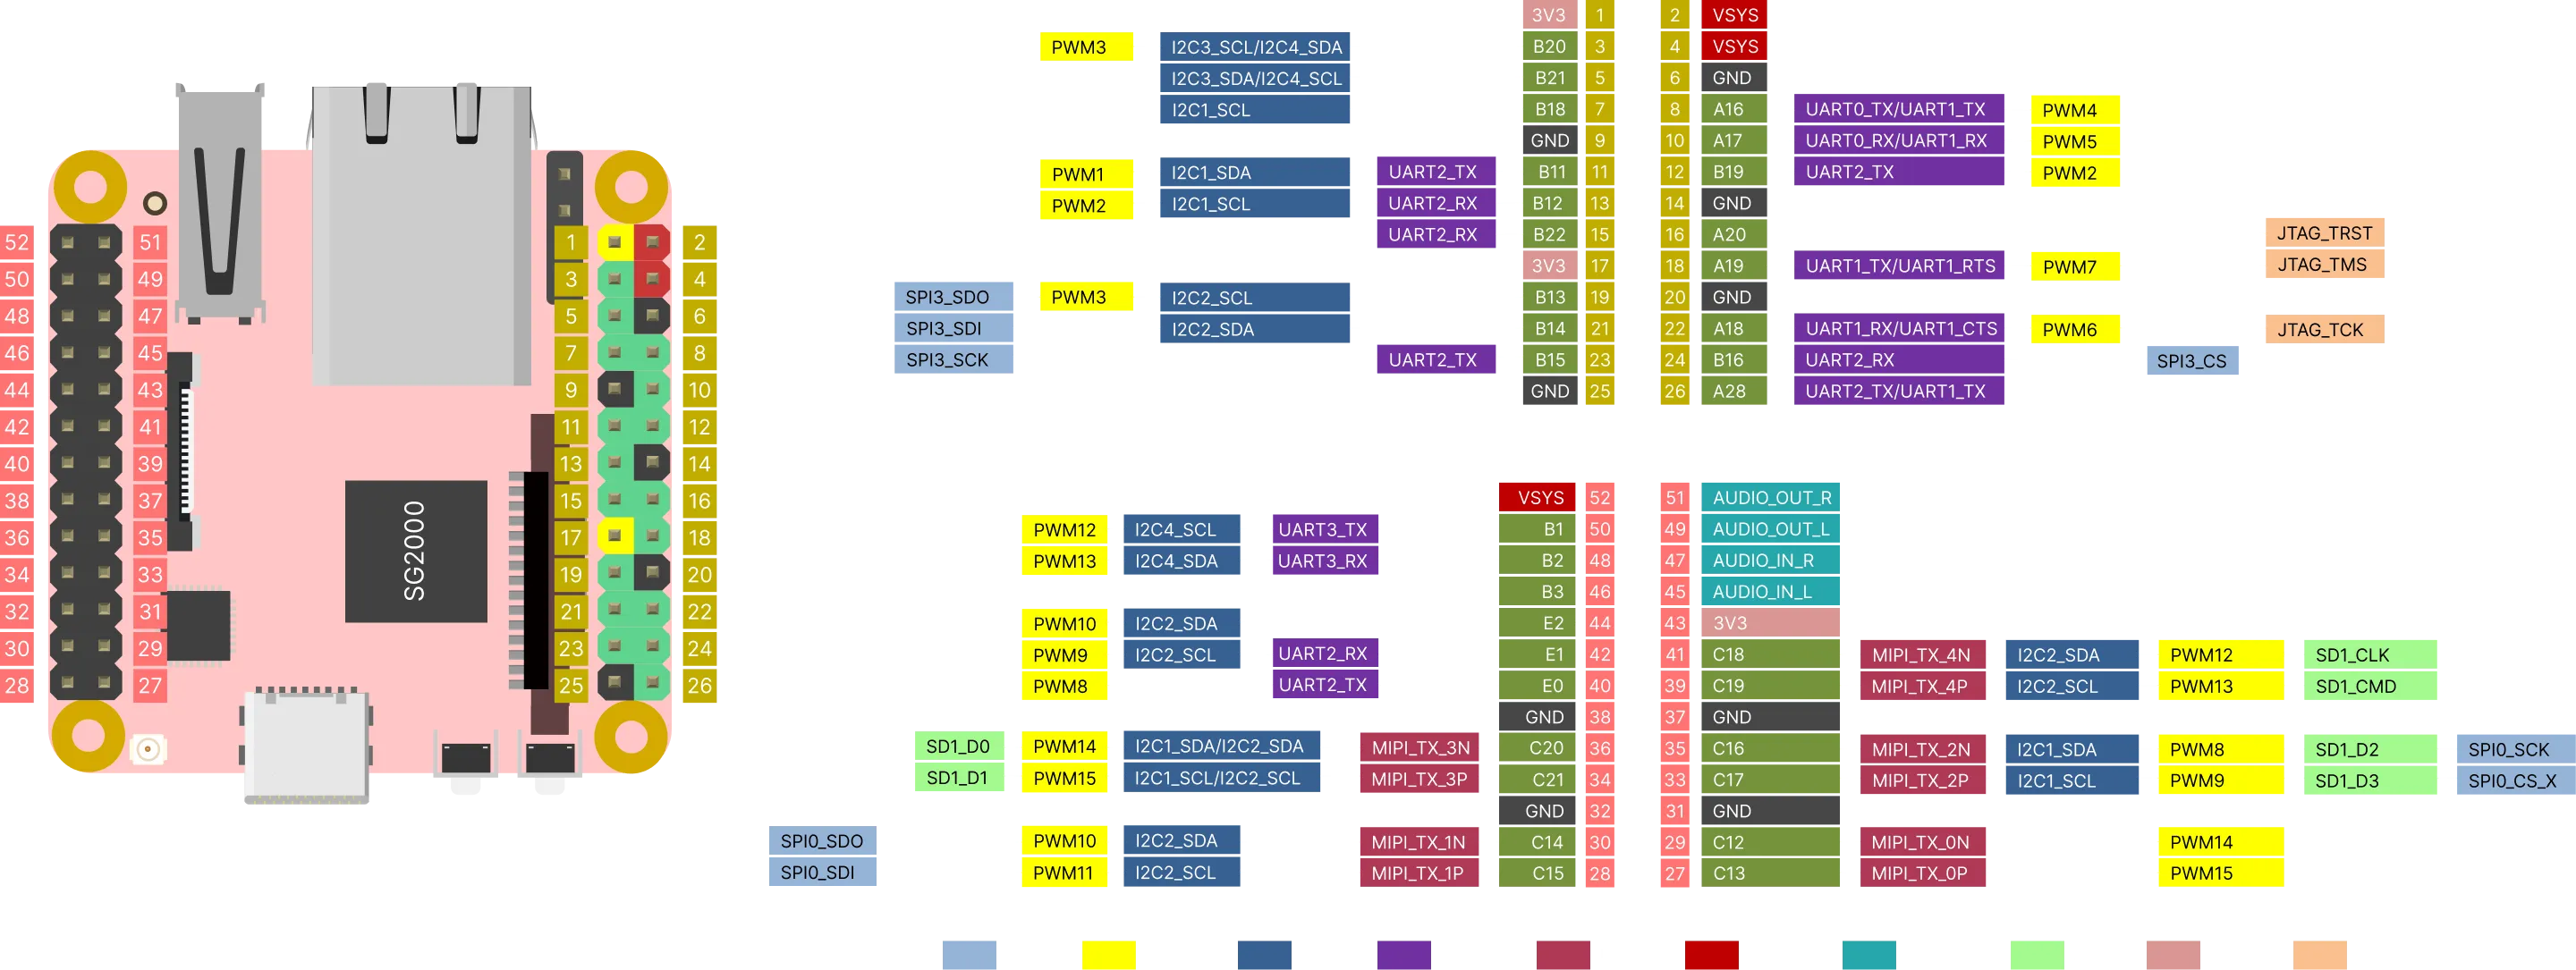
\includegraphics[width=1\linewidth]{images/duos-pinout.png}
    \caption{Pinout Milk-V Duo S} 
    \label{ref:duo-pinout}
\end{figure}
\FloatBarrier
\vspace{1cm}
\section*{Large Language Model}
\addcontentsline{toc}{section}{Large Language Model}
In una sezione del progetto sono stati utilizzati dei Large Language Model (LLM) come \textit{GPT3} (Generative Pre-Training) \cite{GPT3}, \textit{Gemma} \cite{Gemma} e \textit{Mistral} \cite{Mistral}, utilizzati come generatori di gadget. 
\section*{NGINX}
\addcontentsline{toc}{section}{NGINX}
Nel progetto si è anche cercato di riprodurre il risultato presentato nel paper di RiscyROP \cite{RiscyROP}, un generatore automatico di chain per RISC-V e ARM. Per farlo, si è dovuta utilizzare e compilare una versione specifica del webserver NGINX (v1.4.0) \cite{NGINX}, con una specifica \textit{libc} per fare fede all'ambiente citato.\\
Successivamente si è proceduto con l'estrazione di gadget e si è utilizzato GPT3 per cercare di costruire una chain valida per generare un exploit partendo da una nota vulnerabilità di NGINX: \textit{CVE-2013-2028} \cite{NGINXcve}.
\section*{CVA6}
\addcontentsline{toc}{section}{CVA6}
CVA6 \cite{openhwgroup} è una implementazione open-source di un core RISC-V con pipeline a 6 stadi a 64 bit. Supporta la cache e interfacce come AXI che permettono la comunicazione con le periferiche ed è progettato per le alte prestazioni.\\
CVA6 è utilizzato generalmente per scopo di studio, ma può essere esteso anche in prodotto commerciali dato il basso costo implementativo. Di seguito abbiamo la schematica della pipeline a 6 stadi di CVA6.
\vspace{1cm}
\FloatBarrier
\begin{figure}[!htbp]
    \centering
    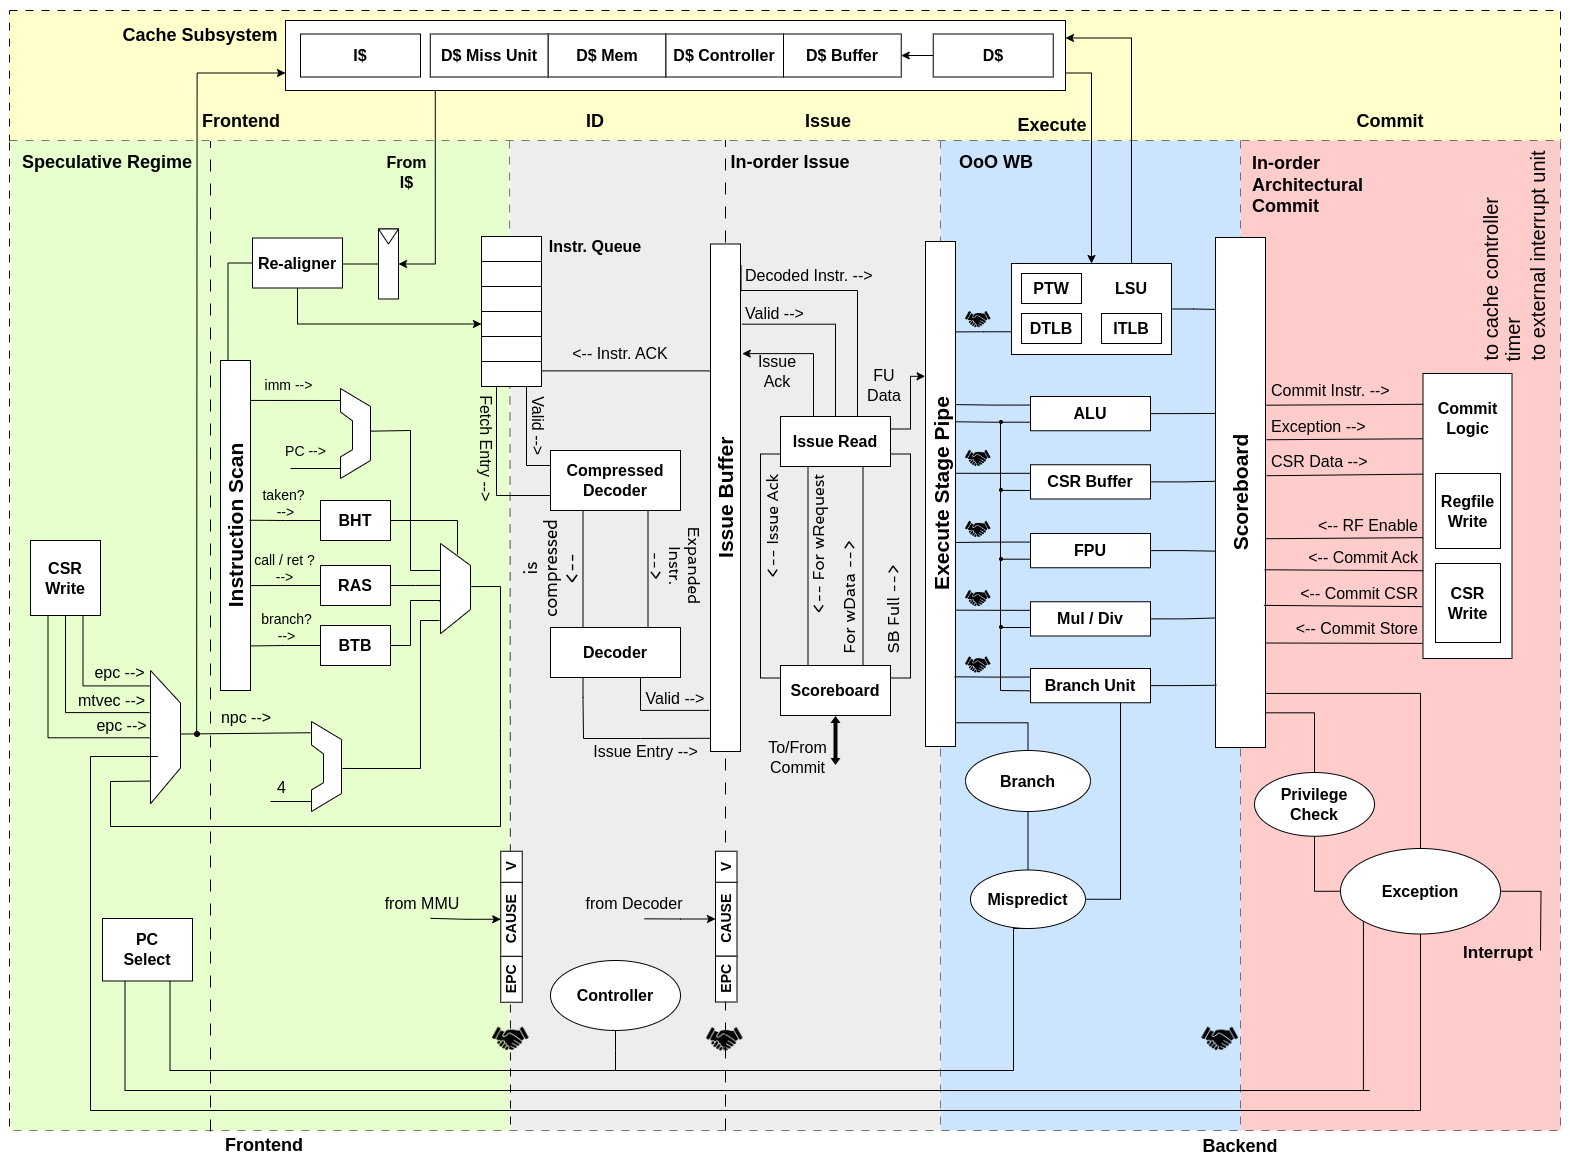
\includegraphics[width=1\linewidth]{images/cva6-scheme.png}
    \caption{CVA6 Pipeline Diagram} 
\end{figure}
\FloatBarrier
\vspace{1cm}
\subsection*{Cheshire}
\addcontentsline{toc}{subsection}{Cheshire}
Cheshire \cite{ottaviano2023cheshire} è una piattaforma minimale basata su sistema Linux in grado di supportare il boot di processi basati su core RISC-V CVA6.
\vspace{1cm}
\FloatBarrier
\begin{figure}[!htbp]
    \centering
    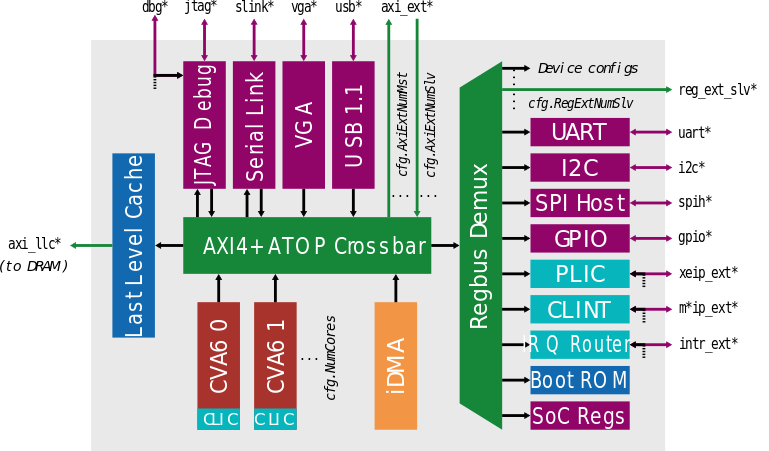
\includegraphics[width=1\linewidth]{images/arch.png}
    \caption{Cheshire architecture} 
\end{figure}
\FloatBarrier
\vspace{1cm}
Durante la fase di testing è stato utilizzato Cheshire per caricare dei programmi contententi vulnerabilità ad hoc e analizzarli tramite meccanismi di Control Flow Integrity, usando il simulatore e facendo dei test direttamente su FPGA.